%!TEX root = foo-thesis.tex


\chapter{Results and Discussion}
\label{chap:results}

This chapter details the performance and quality characteristics of the implemented techniques and  examines their memory usage. For each technique, it will subsequently discuss the up- and downsides and identify alternatives.

\section{Scenes, Settings and Testing System}
\label{sec:results:settings}

The implementation is tested in the Crytek Sponza and San Miguel scene, with 260k and 7.9M triangles respectively, both provided by \citet{McGuire2011Data}.

% no antialiasing but SSAO?

Unless otherwise noted, the parameters used for the measurements and screenshots are:
\begin{outline}
    \1 1920x1080\,px output resolution
    \1 1024 VPLs
    \1 2048\,px² ISM texture, i.\,e.\ 64\,px² per ISM
    \1 Single-pixel point renderer enabled, 16 VPLs considered per point, up to 4 collected
    \1 4x4 interleaving pattern
    \1 Clustered shading: 128\,px² tile size, 16 depth slices
\end{outline}

\noindent
The hardware specification of the testing system is as follows:
\begin{outline}
    \1 Intel Xeon dadada
    \1 NVIDIA GeForce GTX 750 Ti, locked to xxx Mhz for reproducible results
    \1 mainboard?
    \1 other stuff?
\end{outline}

\todo{hardware specifications}

\section{RSM Generation and VPL Sampling}
\label{sec:results:RsmAndVplSampling}
\begin{outline}
\1 RSM generation is the same as G-Buffer generation, possibly with a different resolution. as said earlier, depending on the specific use case, this rendering pass can also render the shadow map.
\1 screenshot of RSM G-buffers

\1 VPL sampling takes fractions of a millisecond and is negligible. bear in mind that in order to achieve high quality levels, a more elaborate sampling algorithms needs to be implemented, which can actually take most of the available time. See \citep{hedman2016sequential} for an advanced sampling algorithm.
\1 screenshots of debug splotches visualized

\1 our sampling pays no attention to relevance to the current frame and wastes budget on lights contributing little or nothing
\1 screenshot of VPLs on the roof

\1 our sampling has the additional downside of poor temporal stability when the scene light moves. this is due to each VPL staying at the exact same position in the light's viewport, so it ``follows'' the light's movements in a certain way, jumping over depth discontinuities along the way.

\1 frame-to-frame coherency here? two screenshots with diff.
\end{outline}


\section{ISM Rendering}

\subsection{Point Rendering with Splatting}




%\Cref{fig:???} shows the Crytek Sponza scene rendered using ISMs created by the splat renderer (a) and the single-pixel renderer (b). A section of the ISM texture is shown for each renderer in the lower row.


\subsubsection{Quality}
\label{sec:results:ism:quality}

\begin{figure}[htb]
\centering
  \begin{tabular}{@{}cc@{}}
    
\includegraphics[width=.48\textwidth]{screenshots/ism_splat_cropped} &
    
\includegraphics[width=.48\textwidth]{screenshots/ism_single_pixel_cropped}
  \end{tabular}
  \caption{ISMs rendered using the splat renderer (left) and single-pixel renderer (right) with default settings. The single-pixel renderer performs interpolation between points, uses more points and doesn't let points ``bleed'' into neighboring ISMs, but takes more time.}
  \label{fig:results:isms}
\end{figure}

\Cref{fig:results:isms} shows a few ISMs rendered with the splat and single-pixel renderer. The imperfections do show, and not only through the low resolutions. The distortion of the surface silhouettes by the splat renderer or postprocessing contribute their part, making it hard to identify which part of the Crytek Sponza is shown.

\begin{figure}[htb]
\centering
  \begin{tabular}{@{}cc@{}}
    \includegraphics[width=.48\textwidth]{screenshots/darkening_splat} &
    \includegraphics[width=.48\textwidth]{screenshots/darkening_single_pixel}
  \end{tabular}
  \caption{Darkening caused by the splat renderer (left) compared to the single-pixel renderer (right). Note that there is no skylight rendered, which leads to an unnaturally dark upper part in the image even for the single-pixel renderer.}
  \label{fig:results:ismDarkening}
\end{figure}

Comparing the screenshots in \cref{fig:results:ismDarkening}, it becomes apparent that the splat renderer causes visible darkening in the upper part of the image. The reason is likely that the point splats are always oriented towards the camera and do not take the point's normal into account when rendering, amplifying the usual aliasing artifacts of common shadow maps. As a result, any point size larger than one pixel causes surfaces that are not directly facing the camera appear nearer than they actually are when doing shadow lookups in the ISMs. A larger shadow bias could compensate for that but would introduce heavier light leaking. Another possibility would be to use the normal to calculate a point's depth per fragment at a potentially high performance cost.

As the single-pixel renderer does not use splats, it does not have this problem. One could say it performs the per-fragment depth calculation implicitly during interpolation in the postprocessing phase.


\begin{figure}[]
\centering
  \begin{tabular}{@{}cc@{}}
    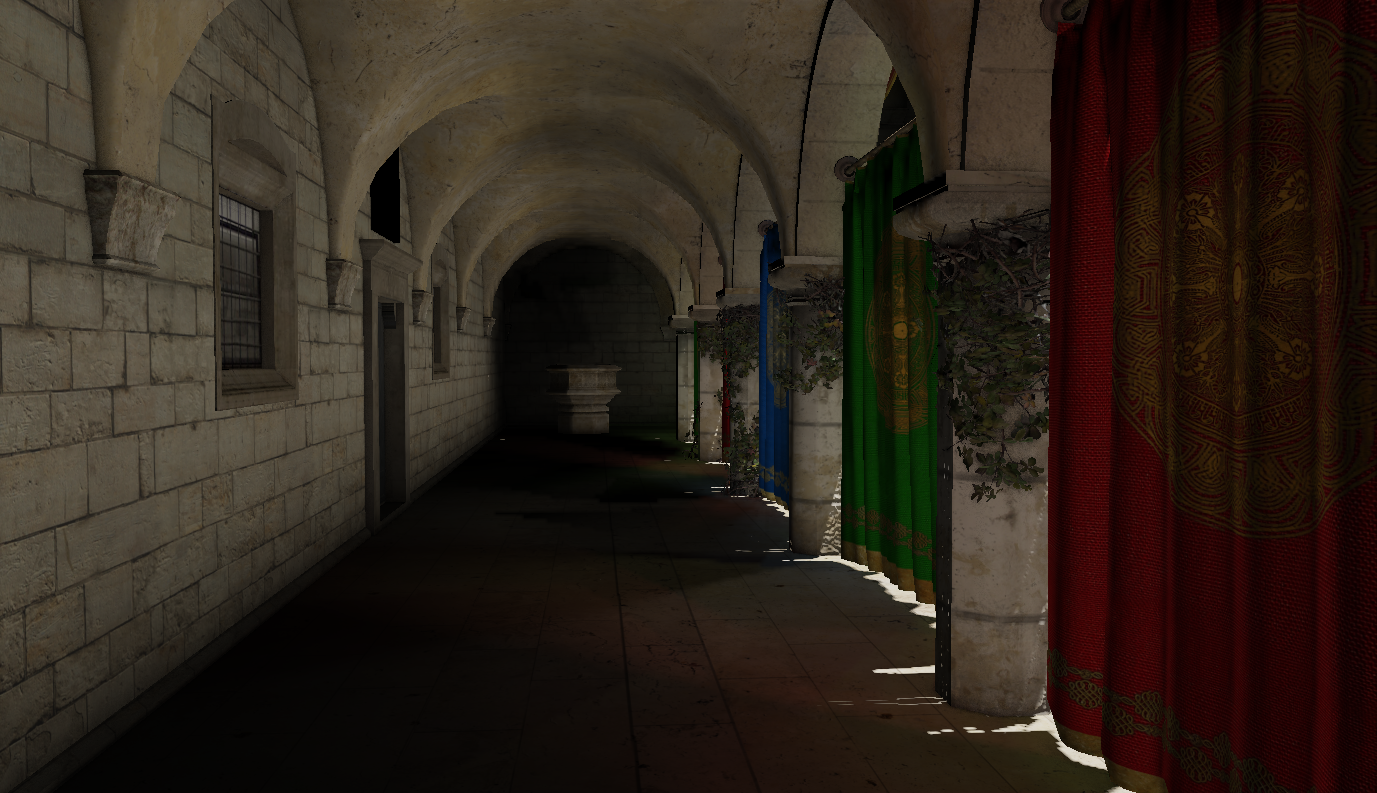
\includegraphics[width=.48\textwidth]{screenshots/leaks_splat} &
    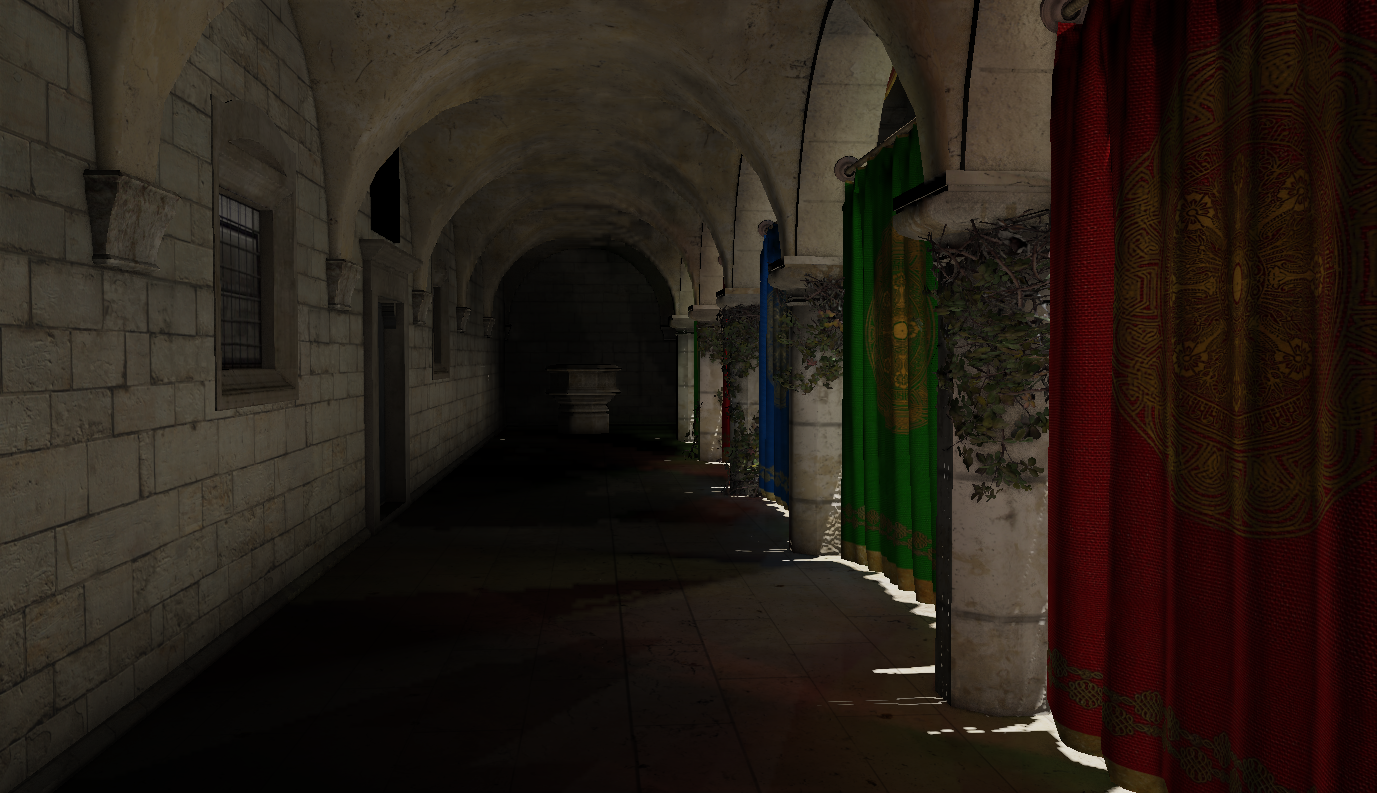
\includegraphics[width=.48\textwidth]{screenshots/leaks_single_pixel}\\
    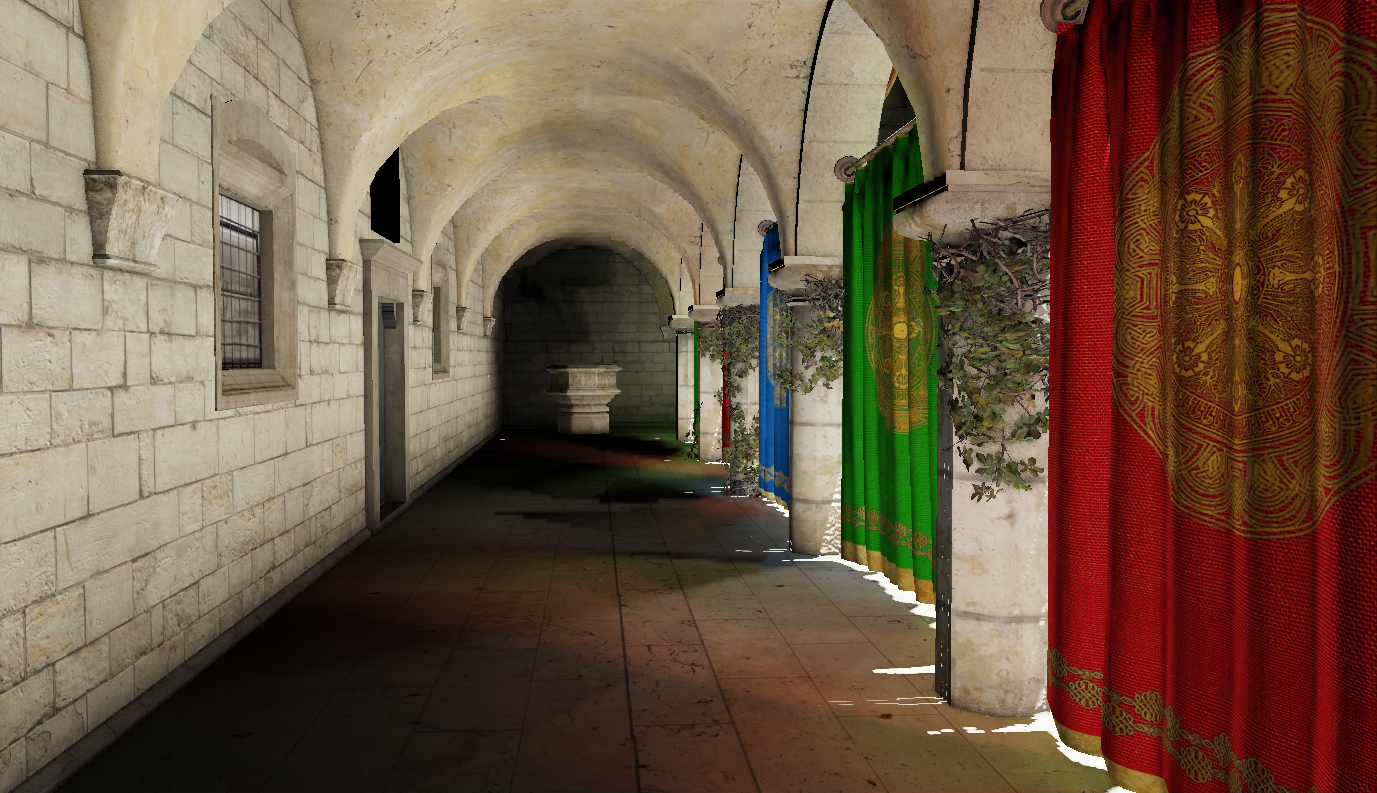
\includegraphics[width=.48\textwidth]{screenshots/leaks_splat_exposure} &
    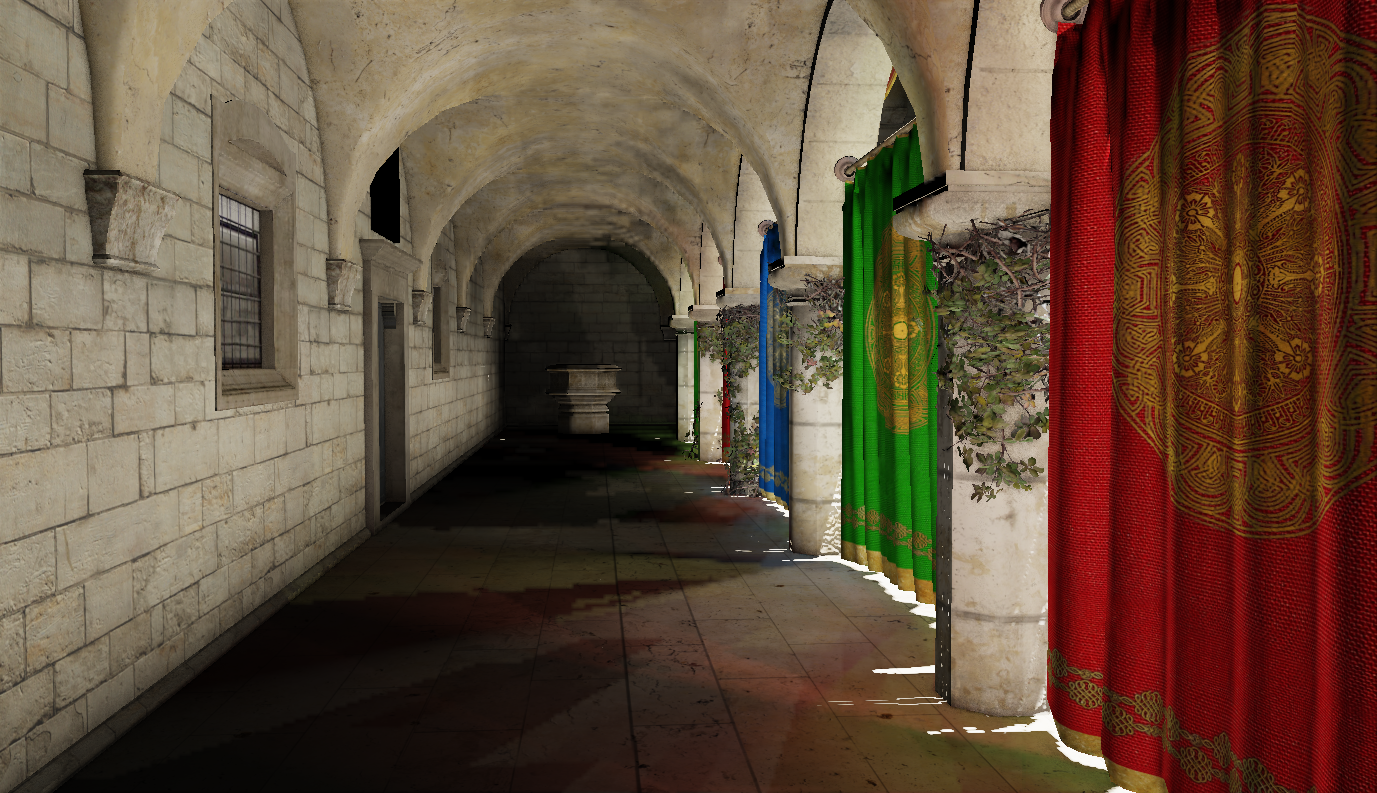
\includegraphics[width=.48\textwidth]{screenshots/leaks_single_pixel_exposure}
  \end{tabular}
  \caption{Light leaks caused by the imperfect shadow maps rendered with the splat renderer (left) and single-pixel renderer (right). VPLs from beneath the curtains leak light onto the wall and ceiling, while VPLs on the pillars and curtains light the floor. The renderings in the bottom row use a higher exposure for illustration. }
  \label{fig:results:leaks}
\end{figure}


\Cref{fig:results:leaks} shows a case the ISM technique has difficulties with. The image should be mostly dark or at least uniformly lit through the small gap below the curtains,instead the wall and ceiling receive a lot of light and the floor displays several artifacts. The root cause is that the VPLs are placed right behind the curtains, so the occluding geometry, i.\,e.\, the curtain, is very near to the light source. Due to the randomness involved when selecting the point set for rendering the ISMs, it often happens that the points near to the light source are rendered into other ISMs, leaving a large hole behind. The single-pixel renderer copes a bit better than the splat renderer since it uses more points, but does not provide a satisfactory result either.



\begin{figure}[]
\centering
  \begin{tabular}{@{}cc@{}}
    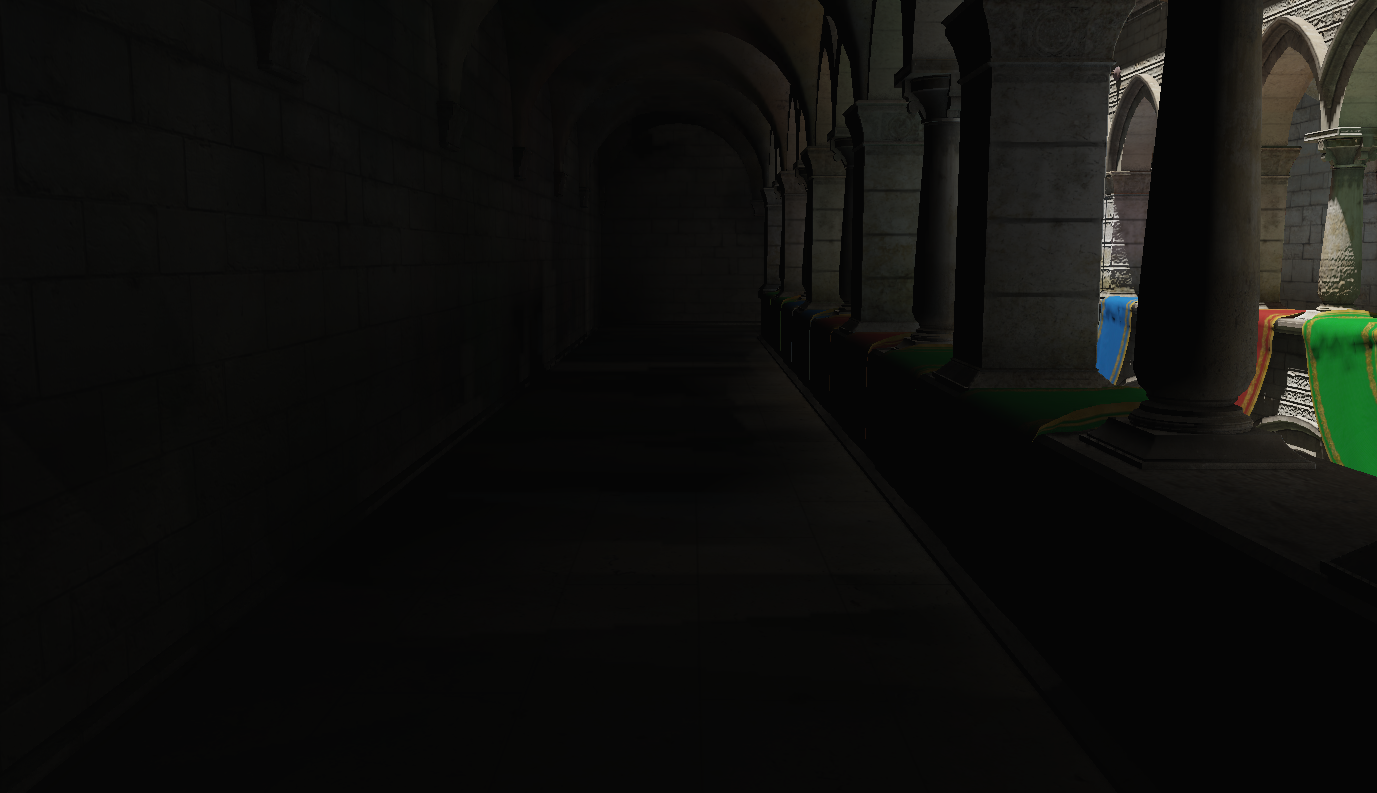
\includegraphics[width=.48\textwidth]{screenshots/bias_splat} &
    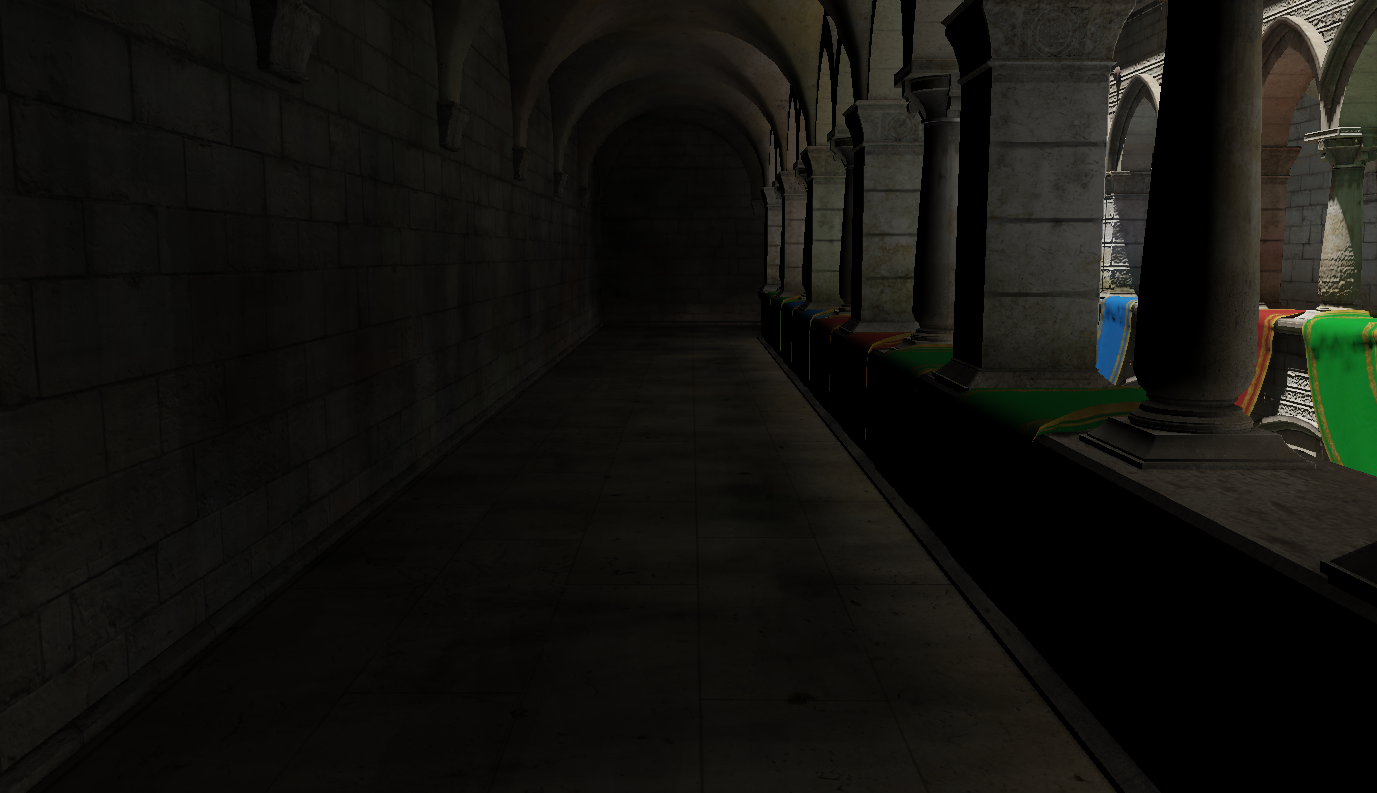
\includegraphics[width=.48\textwidth]{screenshots/bias_single_pixel}\\
      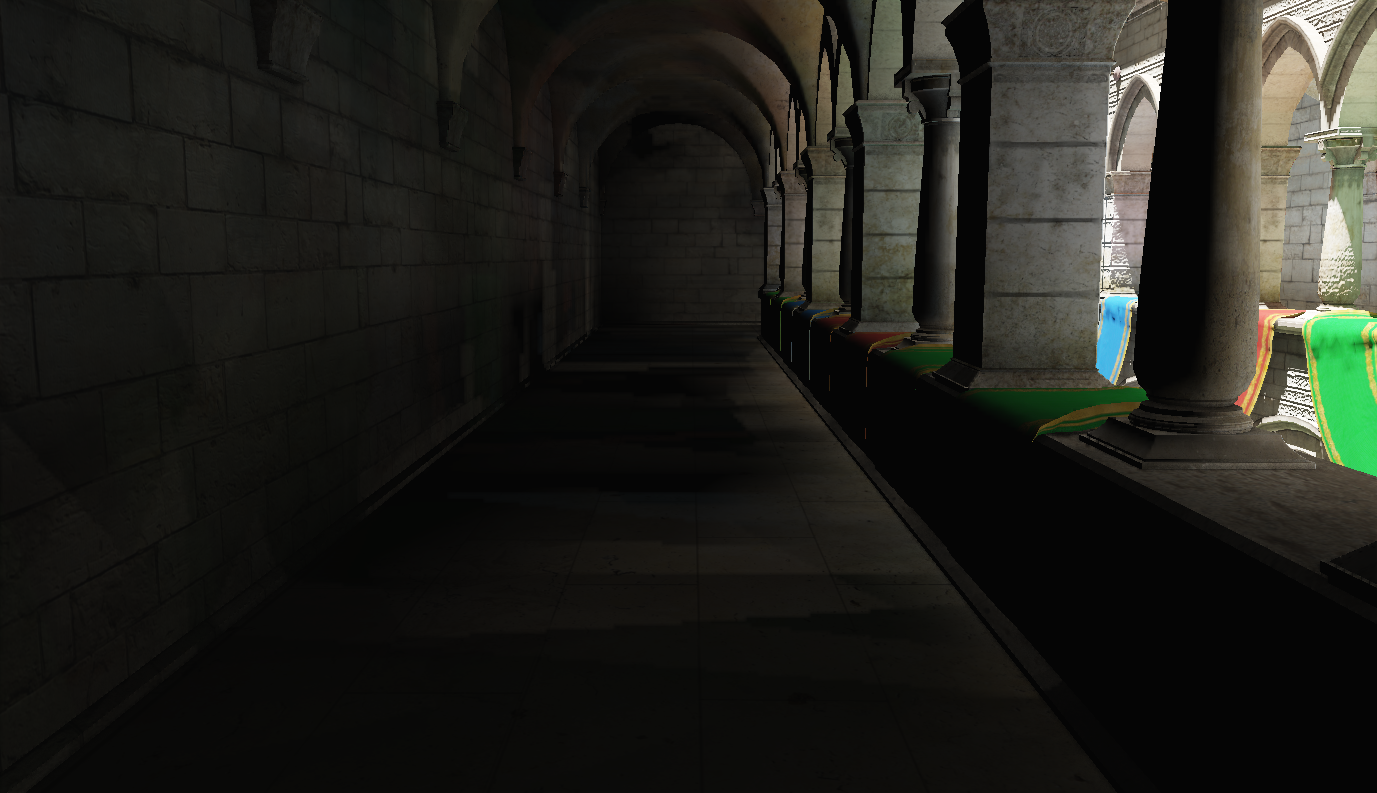
\includegraphics[width=.48\textwidth]{screenshots/bias_splat_exposure} &
      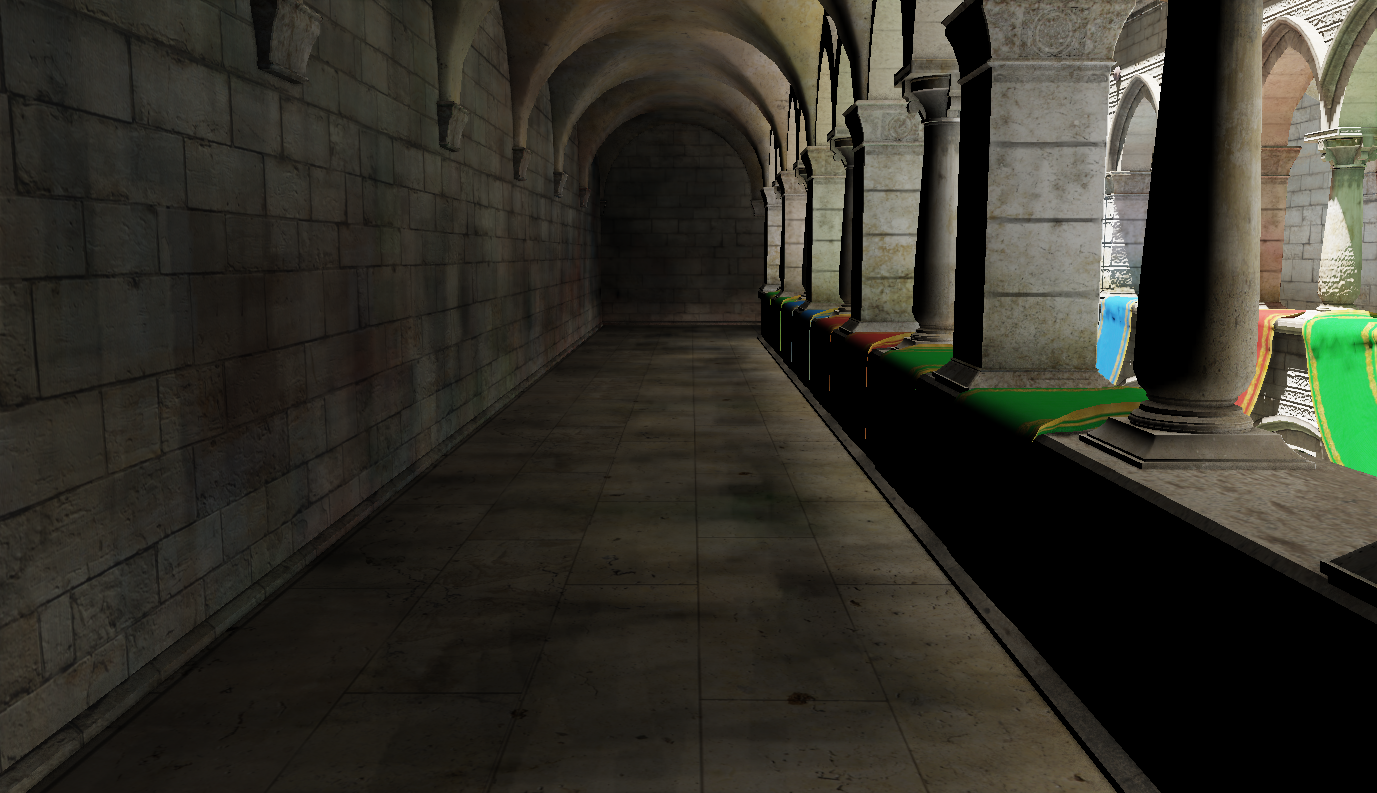
\includegraphics[width=.48\textwidth]{screenshots/bias_single_pixel_exposure}
  \end{tabular}
  \caption{Light leaks caused by using a relatively large shadow bias with the purpose to hide artifacts of the ISMs. The screenshots to the left use the splat renderer, the right ones the single-pixel renderer. Bottom row uses a higher exposure.}
  \label{fig:results:bias}
\end{figure}

Our implementation hides some of the inaccuracies of the ISMs by using a relatively large shadow bias. The resulting light leaks are shown in \Cref{fig:results:bias}. While the splat renderer fares better here, it does so mainly by darkening the whole image since it uses rather large points. The single-pixel renderer on the other hand correctly lets light shine through the columns, but shows a very noisy result on the left wall.


\todo{Screenshots when enlarging the points / making them smaller. Discuss.}

\todo{Screenshots when doing more points. either by tessellation or by collecting more. Discuss.}

\todo[color=yellow]{count point for splat renderer and output them somehow.}

\todo{Compare to max quality}

\todo[color=yellow]{implement max quality. every point into every ISM. likely render everything once for each ISM. a checkbox: when checked, compute high-quality once and don't change. back to normal when unchecked.}

\todo{for single-pixel-renderer: maybe show one full-size shadow map to show this *can* work}


\subsubsection{Performance}
\label{sec:results:ism:performance}

\begin{table}[h]
\begin{center}
    \begin{tabulary}{0.98\textwidth}{| L | L | L | L |}
        \hline
        Splat Default Settings & Single-Pixel Default Settings & Splat with Single-Pixel Settings & Single-Pixel with Splat Settings \\ \hline
        3.4\,ms & 8.5\,ms & 38\,ms & 6.2\,ms \\
        \hline
    \end{tabulary}
    \caption{Timings of the ISM renderers with different settings.}
    \label{tab:results:ism_timings}
\end{center}
\end{table}

\Cref{tab:results:ism_timings} shows the time needed for rendering the ISMs with both renderers and different settings.

Note that the comparison between the two renderers with default settings is not a fair one, since the single-pixel renderer uses more points and performs clamping per default. If the splat renderer is changed to behave similarly, it takes one additional millisecond for the clamping, and 33 additional milliseconds for using the same technique to collect VPLs as the single-pixel renderer does. There are several reasons for this heavy slowdown: First, we implemented this by emitting multiple vertices in the geometry shader, which is known to have poor performance on current GPUs. Second, the additional fillrate and overdraw became an issue when using too many points, a bottleneck that is unlikely to occur when using the single-pixel renderer. And third, while the single-pixel renderer uses shared memory to load the 16 VPLs once, the fragment shader of the splat renderer has no access to shared memory and has to load all 16 VPLs per invocation, creating high register pressure.

Conversely, if the single-pixel renderer does not perform clamping, the push phase needs 0.3\,ms less (2.4\,ms to 2.1\,ms), and when it considers only one VPL per point, the point renderer uses 2.0\,ms less (2.9\,ms to 0.9\,ms).

Since the technique implements no adaptivity, these numbers are independent from the viewport. They are however slightly affected by VPL placement, since it influences culling. In a second scenario, where the sunlight shines directly from above, all VPLs are placed on the floor facing up. As a result, much fewer points are culled during ISM rendering, resulting in slightly higher timings. The splat renderer needed an additional 0.7\,ms, whereas the single-pixel renderer needed only 0.2\,ms more.

\todo{Numbers when enlarging the points / making them smaller. Discuss. Note how the single-pixel renderer is (hopefully) not affected by point size.}

\todo{Numbers when doing more points. either by tessellation or by collecting more. Discuss.}


\subsubsection{Detailed Performance Measurements for the Single-Pixel Point Renderer}
\label{sec:results:ism:performanceSinglePixelRenderer}


\begin{table}[h]
\begin{center}
    \begin{tabulary}{0.98\textwidth}{| L | L | L | L || L |}
        \hline
        Point Collection & Point Rendering & Pull Phase & Push Phase & Total\\ \hline
        2.1\,ms & 3.0\,ms & 1.0\,ms & 2.4\,ms & 8.5\,ms\\
        \hline
    \end{tabulary}
    \caption{Timing breakdown of the single-pixel point renderer.}
    \label{tab:results:timing_breakdown_single_pixel}
\end{center}
\end{table}

\begin{table}[h]
\begin{center}
    \begin{tabulary}{0.98\textwidth}{| L | L | L | L | L | L | L | L || L | L || L |}
        \hline
        PL 1 & PL 2 & PL 3 & PL > 3 & PS > 2 & PS 2 & PS 1 & PS 0 & PL Total & PS Total & Total \\ \hline
        0.57 & 0.34 & 0.10 & 0.04 & 0.09 & 0.19 & 0.71 & 1.47 & 1.05 & 2.46 & 3.5\\
        \hline
    \end{tabulary}
    \caption{Timing breakdown of the pull (PL) and push (PS) phase. The numbers of the individual steps indicate to which mipmap level they write, which is why the pull phase starts with 1 and the push phase has descending numbers. All timings are in milliseconds.}
    \label{tab:results:timing_breakdown_pull_push}
\end{center}
\end{table}


\Cref{tab:results:timing_breakdown_single_pixel} gives more detailed performance measurements of the single-pixel renderer, while \cref{tab:results:timing_breakdown_pull_push} further breaks down the individual steps of the pull and push phase. Note how the timings scale roughly as expected (PL 3 and PS 2 are taking roughly 4 times longer than PL 2 and PS 1, respectively), but not so the first and last step. This is due to the reduced input data size (or output size, respectively), as explained in \cref{sec:impl:pullPushPostprocessing}. Also note how the push phase does take roughly the time of the pull phase if it were not for the last phase, where it writes to the full 2048\,px² of miplevel zero, whereas the first pull phase only writes to the miplevel one with 1024\,px².

\todo{Impact of packing?}

% show this is bandwidth bound. calculation how much memory is read and written, vs bandwidth of GTX 980.
%     - roughly 110MB read and written, that's 1.2ms.
%     - 16MB of that unnecessarily because of the 2nd layer of input texture
%     - By parallel reduction juju reduced by 22MB or 0.2ms.
%     - with more juju, maybe brought down to actually that time, except for the arithmetic stuff of course...


\subsubsection{Memory Usage}
\label{sec:results:ism:memory}

The point splat renderer uses no more memory than the ISM texture itself requires, which is 8\,MB for a 2048\,px² 16-bit depth buffer.

The single-pixel renderer uses additional memory. First, it uses a buffer for storing the points. This is implemented as four-channel 32-bit float texture, with the first three channels containing the position, and the last channel the radius (8 bit) and normal (24 bit, see \cite{Cigolle:2014:NormalPacking}). With a maximum point count of 2048 per ISM (keep in mind they are rendered into multiple ISMs later), this buffer uses 32\,MB.
The additional textures used are the render target of the single-pixel renderer (single-channel 2048x2048x2\,px, 32-bit integer, uses 32\,MB), the mipmap levels used by the pull-push algorithm (two channels, 32-bit, use approx. 11\,MB) and the final ISM (same as used by the splat renderer, uses 8MB).

Added together, the single-pixel renderer uses a total of 83\,MB, likely with room for optimization left.


\subsubsection{Problems with High Geometric Density}
\label{sec:results:ism:densityProblems}

As a more demanding test case the San Miguel scene with 7.9M triangles. The most apparent problem of the presented implementation is the lack of adaptivity to the current viewport and VPL positions in addition to the lack of LOD methods. As a result, all 7.9M triangles are used every frame to render the ISMs, with corresponding performance results.

Screenshots with the San Miguel scene

Quality also suffers. Not tuned to such small triangles.

Numbers


\subsection{Comparison of the Splat and Single-Pixel Renderer}
\label{sec:results:ism:comparison}


The single-pixel renderer provides numerous advantages over the splat renderer. Using a compute shader to render the points lifts the restrictions of the fixed-function pipeline and e.\,g.\ enables rendering each point into multiple ISMs without large performance losses. Quality-wise, it can reproduce surfaces more accurately by correctly interpolating between points.

The drawbacks obviously include the additional rendering time and memory. Besides, the added complexity should not be underestimated. Specifically, we found it hard to fine-tune the pull-push algorithm to give us satisfactory results, especially in the face of the low resolutions of ISMs and the limited data available for reconstruction after selecting a random and sparse set of points.

\todo{Add notes about scaling when i have point counts}



\subsection{Discussion}
\label{sec:results:ism:discussion}

Imperfect shadow maps have several deficits, some of which are inherent to the technique and difficult to solve, others are specific to the implementation choices and tradeoffs in our implementation and might be easier to overcome.

First, ISMs reduce the scene's geometry to points. At the resolution that is achievable in a real-time budget, this is already a stark approximation that loses a lot of accuracy.

Second, because a sparse set of points is used for each ISM, each point must be enlarged to accomodate for the neighboring points that are likely missing in the chosen ISM. For instance, if an area is represented by a thousand points and only one tenth of all points is used for each ISM, each remaining point's area must be enlarged by a factor of ten to result in an equally large area in the rendered output. Of course, this approach leads to deformed geometry since points at the edges of the area get enlarged as well, growing over the borders of the original geometry.

Third, there are also numerical issues. For instance, both the splatting and postprocessing approaches ignore the distortion caused by the projection, and thus might render even simple surfaces incorrectly. This contributes to the necessity of using a relatively large shadow bias. This can likely be solved, albeit at the cost of additional complexity.

Fourth, and this is in our view the most important shortcoming, ISMs handle geometry in the vicinity to VPLs badly as can be seen in \cref{fig:results:leaks}. To sufficiently approximate such surfaces when rendering ISMs, one would need to greatly increase the number of points created near VPLs, possibly in addition to stepping away from using a fully random approach for point selection and select a specific point set for each ISM depending on the VPLs location.

As for most global illumination algorithms, a massive improvement would be to differentiate between large-scale scene geometry that is important for diffuse light bounces, and smaller geometry of lesser importance. While the latter can possibly be ignored altogether with only minor losses in quality, the shape of large-scale geometry is all the more important to preserve (relatively) precisely.

The San Miguel scene is a good example for this: While the small detail work like dishes and small plants make up most of the geometry and thus most of the rendering time, they contribute only very little to global illumination. This is where our implementation suffers most from the lack of level-of-detail methods.




\section{Interleaved Shading with Compute Shaders}
\label{sec:results:interleavedShading}

\begin{outline}
\1 performance
\1 1x1 and 4x4, if i'm good also 2x2 and 8x8...
\1 quality
    \2 screenshots with and without, with details on e.g. foliage, diffimage? and shaded result
\1 memory usage
    \2 one additional buffer
\1 discussion

\end{outline}

\todo[color=blue]{interleaved shading results}


\section{Clustered Deferred Shading}
\label{sec:results:clusteredShading}

\begin{outline}
\1 parameters: cluster size
\1 performance: time used by additional steps vs saved in GI step
\1 quality: exactly the same
\1 memory usage for the one intermediate result and the light lists buffer
\1 performance of tiled shading. comparable, no memory usage, easier to implement, but less flexible.
\1 discussion
\end{outline}


\todo[color=blue]{clustered deferred shading results}


- one 4k test?
